%%%%%%%%%%%%%%%%%%%%%%%%%%%%%%%%%%%%%%%%%
% Short Sectioned Assignment LaTeX Template Version 1.0 (5/5/12)
% This template has been downloaded from: http://www.LaTeXTemplates.com
% Original author:  Frits Wenneker (http://www.howtotex.com)
% License: CC BY-NC-SA 3.0 (http://creativecommons.org/licenses/by-nc-sa/3.0/)
%%%%%%%%%%%%%%%%%%%%%%%%%%%%%%%%%%%%%%%%%

%----------------------------------------------------------------------------------------
%	PACKAGES AND OTHER DOCUMENT CONFIGURATIONS
%----------------------------------------------------------------------------------------

\documentclass[paper=a4, fontsize=11pt]{scrartcl} % A4 paper and 11pt font size

% ---- Entrada y salida de texto -----

%\usepackage[T1]{fontenc} % Use 8-bit encoding that has 256 glyphs
\usepackage[utf8]{inputenc}
\usepackage[T1]{fontenc}

\usepackage{mathptmx}
\usepackage{fourier}  % Use the Adobe Utopia font for the document - comment this line to return to the LaTeX default

% ---- Idioma --------

\usepackage[spanish, es-tabla]{babel} % Selecciona el español para palabras introducidas automáticamente, p.ej. "septiembre" en la fecha y especifica que se use la palabra Tabla en vez de Cuadro

% ---- Otros paquetes ----

\usepackage{url} % ,href} %para incluir URLs e hipervínculos dentro del texto (aunque hay que instalar href)
\usepackage{amsmath,amsfonts,amsthm} % Math packages
%\usepackage{graphics,graphicx, floatrow} %para incluir imágenes y notas en las imágenes
\usepackage{graphics,graphicx, float} %para incluir imágenes y colocarlas
\graphicspath{ {images/} }
\usepackage{subfig}

\usepackage{algorithm}
\usepackage{algpseudocode}

\usepackage{wrapfig}

% Para hacer tablas comlejas
\usepackage{multirow}
%\usepackage{threeparttable}

%\usepackage{sectsty} % Allows customizing section commands
%\allsectionsfont{\centering \normalfont\scshape} % Make all sections centered, the default font and small caps

\usepackage{fancyhdr} % Custom headers and footers
\pagestyle{fancyplain} % Makes all pages in the document conform to the custom headers and footers
\fancyhead{} % No page header - if you want one, create it in the same way as the footers below
\fancyfoot[L]{} % Empty left footer
\fancyfoot[C]{} % Empty center footer
\fancyfoot[R]{\thepage} % Page numbering for right footer
\renewcommand{\headrulewidth}{0pt} % Remove header underlines
\renewcommand{\footrulewidth}{0pt} % Remove footer underlines
\setlength{\headheight}{13.6pt} % Customize the height of the header

\numberwithin{equation}{section} % Number equations within sections (i.e. 1.1, 1.2, 2.1, 2.2 instead of 1, 2, 3, 4)
\numberwithin{figure}{section} % Number figures within sections (i.e. 1.1, 1.2, 2.1, 2.2 instead of 1, 2, 3, 4)
\numberwithin{table}{section} % Number tables within sections (i.e. 1.1, 1.2, 2.1, 2.2 instead of 1, 2, 3, 4)

\setlength\parindent{0pt} % Removes all indentation from paragraphs - comment this line for an assignment with lots of text

\newcommand{\horrule}[1]{\rule{\linewidth}{#1}} % Create horizontal rule command with 1 argument of height

\usepackage{listings}

\everymath{\displaystyle}
%----------------------------------------------------------------------------------------
%	TÍTULO Y DATOS DEL ALUMNO
%----------------------------------------------------------------------------------------

\title{	
\normalfont \normalsize 
\textsc{\textbf{Desarrollo de sistemas Distribuidos} \\ Grado en Ingeniería Informática \\ Universidad de Granada} \\ [25pt] % Your university, school and/or department name(s)
\horrule{0.5pt} \\[0.4cm] % Thin top horizontal rule
\huge Formal Methods in Software Engineering: \\ % The assignment title
Resumen charla impartida por María del Mar Gallardo 
\horrule{2pt} \\[0.5cm] % Thick bottom horizontal rule
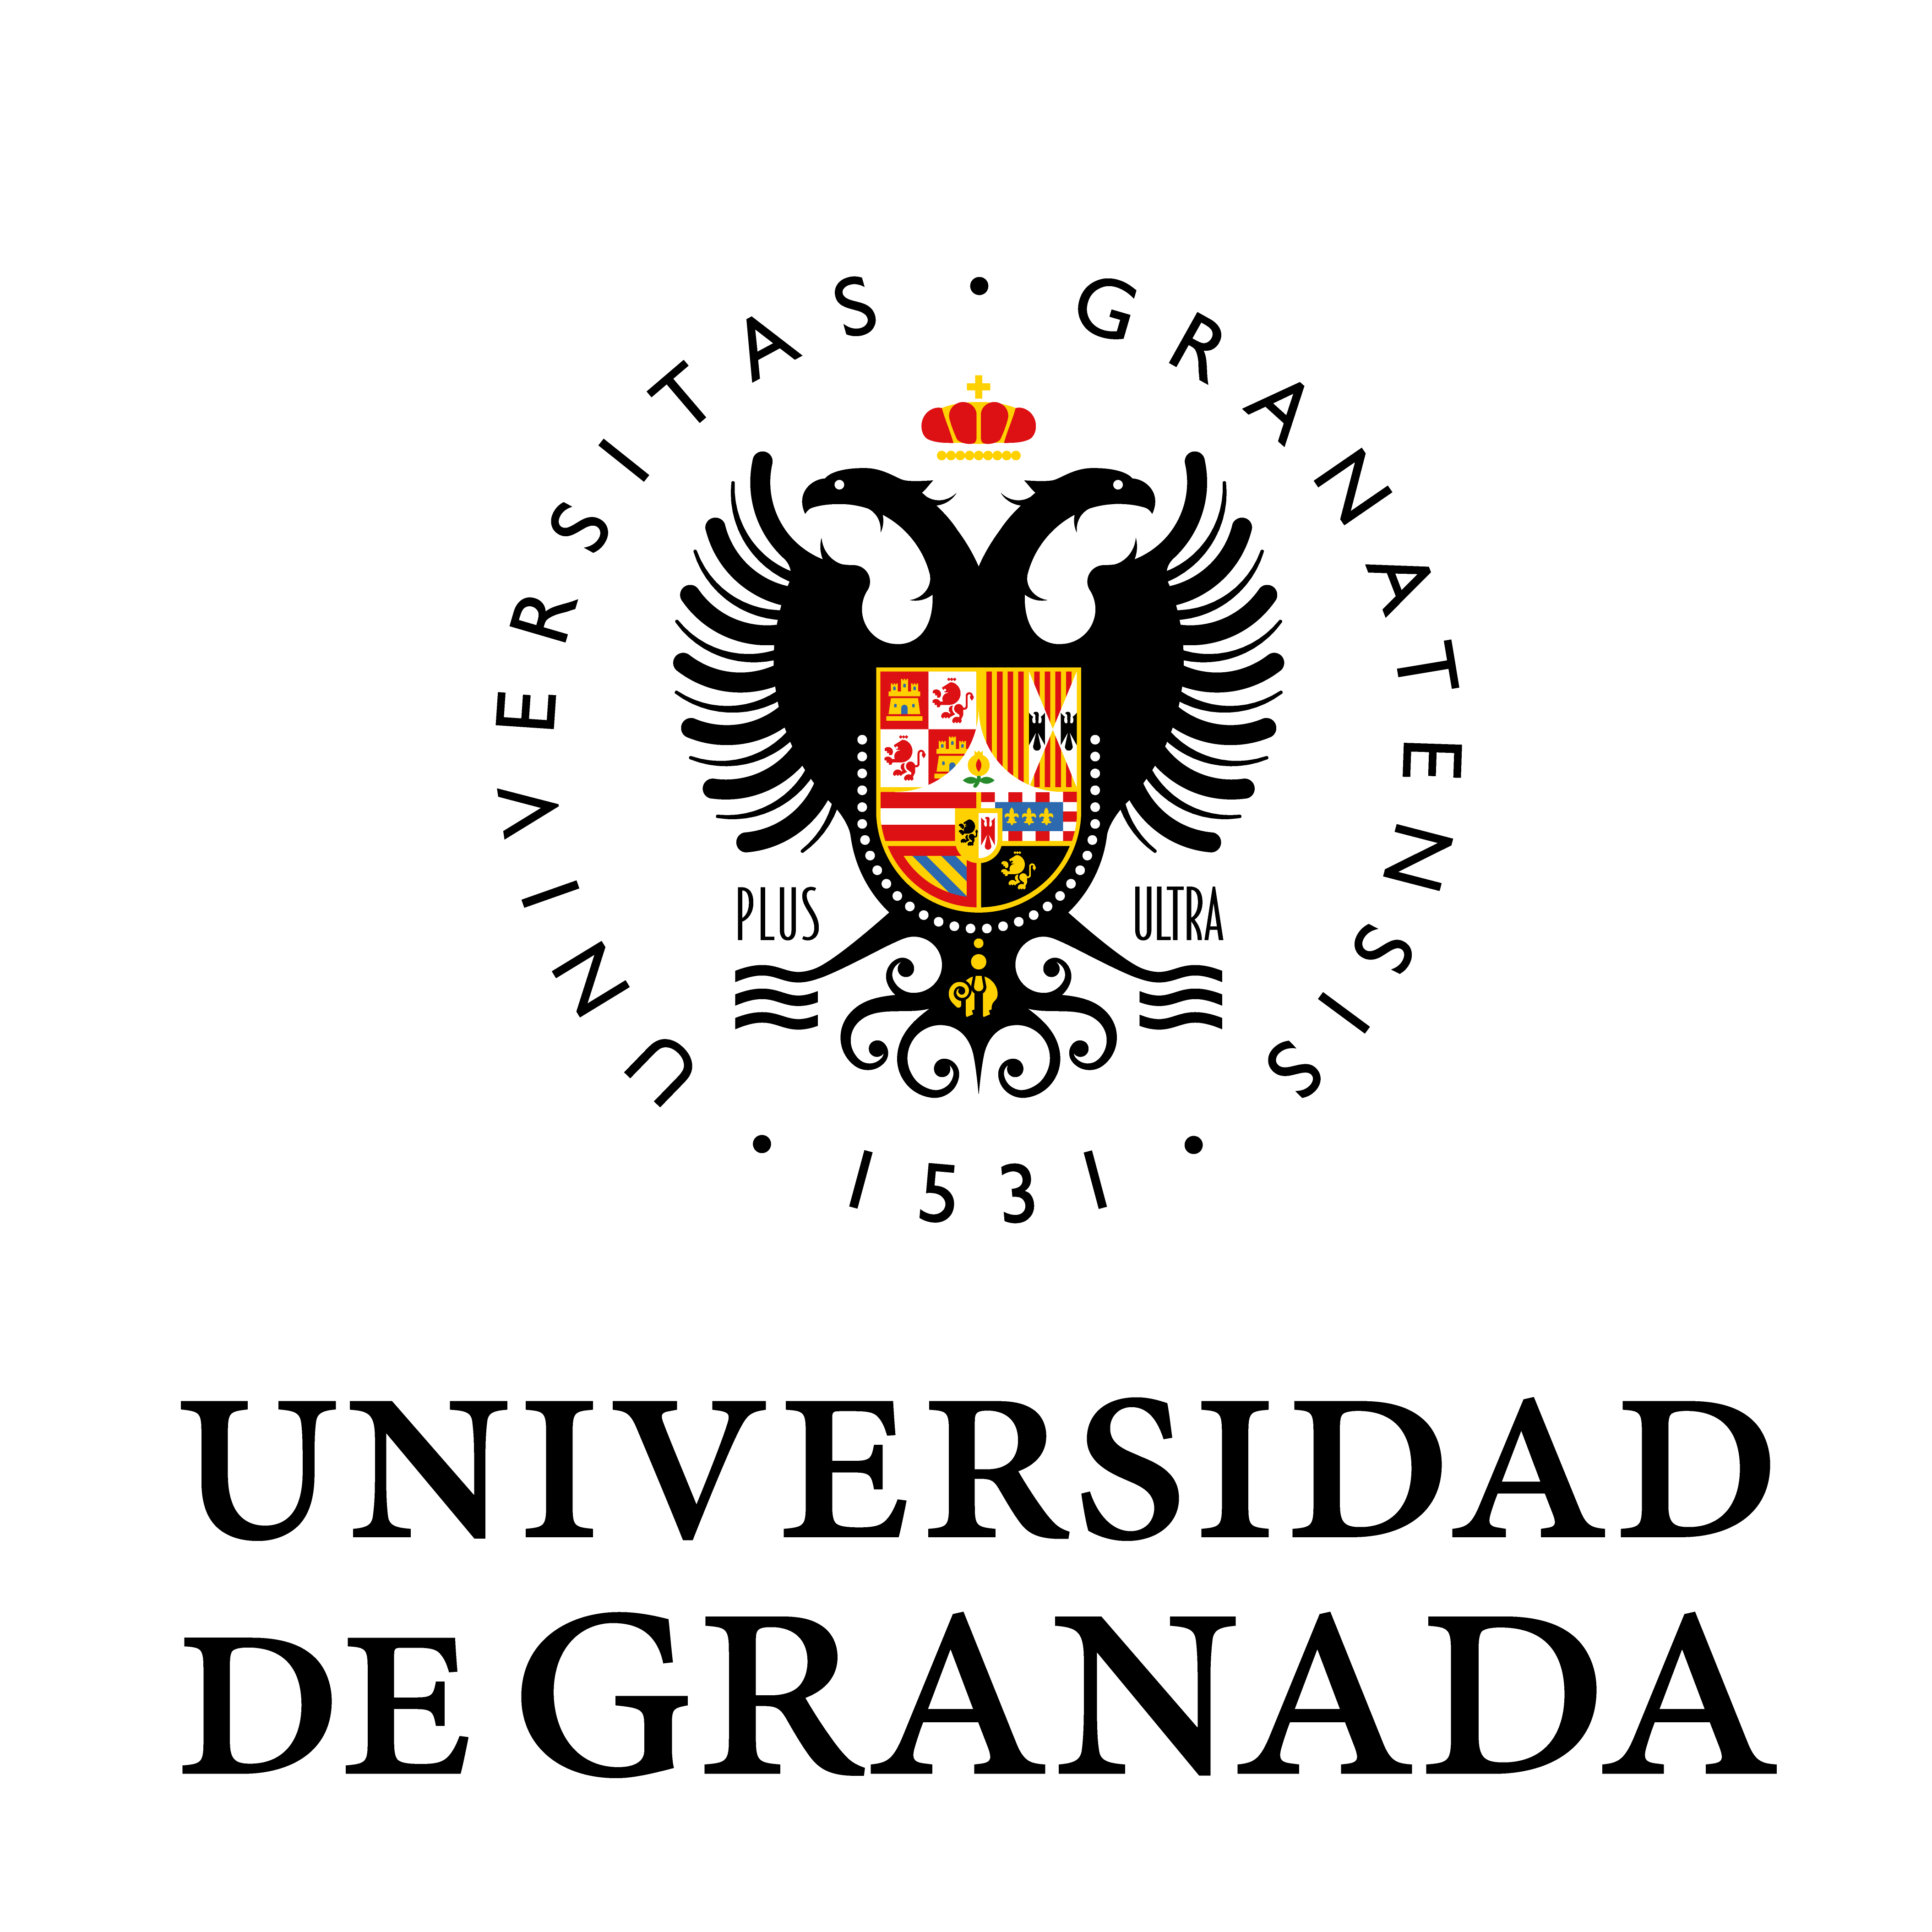
\includegraphics[width=5cm]{logo}\\[8ex]
}




\author{José Luis Molina Aguilar} % Nombre y apellidos

\date{\normalsize\today} % Incluye la fecha actual


%----------------------------------------------------------------------------------------
% DOCUMENTO
%----------------------------------------------------------------------------------------

\begin{document}


\maketitle % Muestra el Título
  \begin{large}
    \centering
  \vfill
  
  Curso 2022-2023\\
  Correo : joselu201@correo.ugr.es
  \vfill
  \end{large}
\newpage %inserta un salto de página

\tableofcontents % para generar el índice de contenidos

%\listoftables -----------------------------------------------------------


\newpage



%----------------------------------------------------------------------------------------
%	Cuestión 1
%----------------------------------------------------------------------------------------
\newpage
\section{Introduccion}

Los métodos formales son un conjunto de técnicas rigurosas y sistemáticas utilizadas para el análisis y diseño de software, que se basan en principios matemáticos y lógicos. Estos métodos permiten la verificación y validación de las propiedades funcionales y no funcionales del software, garantizando que el software cumpla con los requisitos establecidos y sea correcto.

Los orígenes de los métodos formales se remontan a los trabajos de Dijkstra y Hoare, dos pioneros en el campo de la programación y la informática teórica. En la época en que se desarrollaron estos métodos, las técnicas de programación eran más secuenciales y las herramientas no eran tan potentes como en la actualidad.

Sin embargo, a medida que las tecnologías de la información se han desarrollado, los métodos formales han evolucionado para satisfacer las necesidades de los desarrolladores de software modernos. En la actualidad, los métodos formales son cada vez más utilizados en el desarrollo de sistemas críticos, como los sistemas de control aéreo y los sistemas de seguridad informática. 

\section{Model Checking}

No todo el software es absolutamente correcto, siempre existe la posibilidad de 
encontrar fallos, y por eso hay que estar muy atento a los software de sistemas 
críticos para ser examidanos de forma exhaustiva,

la dificultad del análisis de código ha ido incrementándose ya que el SW ha ido 
evolucionando y aumentando, actualmente cualquier dispositivo tiene una gran 
cantidad de código detrás.

Otra fuente de complejidad a la hora de analizar código es la concurrencia, 
las hebras de cada procesador ejecutando simultáneamente son muy difíciles de 
predecir, existe procedimientos que analiza todos los posibles casos y los saca a la luz.

Los autores de la técnica fueron Clarke, Emerson y de forma paralela con otros 
investigadores de otros partes del mundo.

Model checking es una técnica automática que da un numero finitos de estado (M) 
para el modelo del sistema y una propiedad formal (f), y básicamente vemos si un 
programa satisface unas prioridades propuestas a priori, esto lo hacemos 
basándonos en teoría de conjuntos. 
\newline

M satisface f si el conjunto de f es un subconjunto de M.

también se puede comprobar con la negación de los conjuntos que en ciertos casos 
es mas factible de analizar 

Otro punto de vista desde el que partir es ignorando la teoría de conjuntos y 
partir desde una base algorítmica

\subsection{Requisitos para la Aplicación de Model Checking}

Para aplicar el MC necesitamos specification, modelling, simulation

\begin{itemize}
  \item Modeling: el sistema M puede ser analizado mediante Modeling Language
  \item Specifying: Una vez que se tiene el modelo, se debe definir qué propiedades se quieren verificar. Estas propiedades se definen mediante especificaciones formales. Las especificaciones pueden ser expresadas en algún lenguaje de especificación formal, como por ejemplo lógica temporal o lógica de predicados. Las especificaciones deben ser claras y precisas, para que puedan ser utilizadas para verificar el modelo.
  \item Verificar: Una vez que se tienen el modelo y las especificaciones, se puede utilizar la técnica de Model Checking para verificar si el modelo cumple con las especificaciones. La verificación se realiza mediante la exploración exhaustiva del espacio de estados del modelo, lo que implica probar todas las posibles combinaciones de valores de entrada y estados internos del sistema. Esta exploración se realiza de forma automática, utilizando herramientas de software especializadas en Model Checking.
\end{itemize}

\subsection{Transition system}
Secuencial, concurrent and distributed system pueden ser descritos con Labelled Transitions System (LTSs)

Clásico problema para determinar que proceso entra a la sección critica \\
bool  f0,f1 = false;\\

Process P1: \\
 do\\
   f0 = true;\\
   !f1;       \\
   //sc       \\
   f0 = false;\\
        
Process P2: \\
  Inverso   \\
  \newline
Si generamos un grado para ver los posibles entrelazamientos, podemos ver que 
hay estados cíclicos que son correctos mientras que tmb vemos lugares en los que 
llegamos a interbloqueo.

Ahora probemos el programa y vemos que existe una secuencia de operaciones que 
fácilmente nos da un interbloqueo

Utilizamos en la pestaña de verificación del programa una secuencia de 
instrucciones para ver si llegan a interbloque y efectivamente 

\subsection{LTL: Intuitive Semantics }

La semántica de LTL se basa en la noción de "camino" o "trayectoria". 
Un camino es una secuencia infinita de eventos que ocurren en el tiempo, 
y que representa una posible ejecución del sistema. Cada camino se puede 
interpretar como una línea temporal, donde cada punto representa un momento 
en el tiempo y cada evento representa un cambio en el estado del sistema.



\end{document}
